\subsection{Instruction Set Architecture}\label{subsec: processor-instructions-executor}
OlaVM设计指令地址和内存地址在同一空间访问。因为目前虚拟机的空间足够使用,而使用统一空间对于存储进行约束时的列可以更小,减少开销。

\subsubsection{register}\label{subsec: processor-register}
目前在设计ZKVM memory hierarchy的L0层时,业内主要有两种模型,一种是寄存器模型,一种是stack模型。
对于stack模型,状态的更新是按照stack的先进后出模型实现。对于约束的设计相对简洁。
但是缺点是状态的访问不友好,不能随机访问stack中的某个地址的数据,对于寄存器模型只需要一条指令完成的读取操作,stack模型需要多次进行pop和push的操作。或者为了提高效率,如miden的设计中增加swap类指令辅助完成stack内数据访问。
对于register模型,可以随机访问任意寄存器。但是缺点是约束模型需要对上下指令进行copy约束,证明的开销比stack大。

像白皮书设计的那样,OlaVM选择的是寄存器模型。there are 9 general-purpose registers.
符号表示为:$\texttt{r}_0 - \texttt{r}_{8}$。
其中的$\texttt{r}_{8}$作为$\texttt{fp}$(frame pointer)。$\texttt{fp}$为$\texttt{r}_{8}$的别名。

pc指针加载程序后初始指向地址0的指令。之后pc指向的地址值随着指令的执行改变。在没执行jump指令和call指令时,每执行一条指令,如果指令没有使用立即数,pc寄存器里的地址加1,否则加2。

\subsubsection{Olavm instructions}\label{subsec: processor-instructions-executor-instructions}
为了尽量减少约束的degree。OlaVM选用了精简的指令集。

Olavm 采用 Word(位宽) = 64bits对指令编码。
一条指令通过一个opcode和最多三个操作数来编码,操作数可以是寄存器名称,也可以是立即数,一个指令编码由下面的8个fields组成。
\begin{itemize}
    \item Field1: 字段名称NULL。占1 bit,不使用。
    \item Field2: 字段名称OP1 immediate flag(OP1\_IMM, imm)。包含1 bit, 如果是0,表示A是一个寄存器名称,如果是1表示这是一个立即数。
    \item Field3: 字段名称operation0 register(OP0\_REG, reg\_src1)。指示使用源寄存器0的序号,包含了9 bits,分别指示0-8共9个寄存器,bit值为1代表本指令使用该序号OP0 寄存器,为0则不使用。
    \item Field4: 字段名称operation1 register(OP1\_REG, reg\_src2)。指示使用源寄存器1的序号,包含了9 bits,分别指示0-8共9个寄存器,bit值为1代表本指令使用该序号OP1 寄存器,为0则不使用。
    \item Field5: 字段名称destination register(DST\_REG, reg\_dst)。指示目标寄存器的序号, 包含了9 bits,分别指示0-8共9个寄存器,bit值置为1代表本指令使用该序号DST 寄存器,为0则不使用。
    \item Field6: 字段名称opcode selector(opcode\_sel)。指示指令的opcode,包含了19 bits,分别指示ISA支持的19种指令,bit值置为1代表本指令使用该opcode,为0则不使用。
    \item Field7: 字段名称padding bits(paddings)。这个filed一共有16 bits。所有bit使用0进行填充,后续可以扩充定义别的字段。
    \item Field8: 字段名称字段名称immediate data(immediate)。这个field会根据field2字段决定是否存在,如果filed2值为1,这个字段将存在一个立即数值,这个字段是2 Word。
\end{itemize}

OlaVM的指令集定义如下表, A表示可能是立即数或者寄存器:
\begin{table}[!ht]
    \resizebox{\textwidth}{!}{%
        \begin{tabular}{|c|c|c|c|c|}
            \hline
            \textit{Type}  & \textit{Instruction} & \textit{Operands} & \textit{Description} & \textit{flag} \\ \hline
            \multirow{2}{*}{Field Operation}  & ADD & ri rj A & Compute rj + A and store the result in ri &   \\ \cline{2-5}
            & MUL & ri rj A & Compute rj * A and store the the result in ri &  \\ \cline{2-5}
            & NOT & ri A &  Compute not A and store the the result in ri &  \\  \hline
            \multirow{2}{*}{Cmp}  & EQ & ri rj A & Equality comparison and store the the result in ri & rj = A \\ \cline{2-5}
            & NEQ & ri rj A &  check whether rj is not equal A and store the the result in ri & rj != A \\ \cline{2-5}
            & ASSERT & ri  A & Assert ri == A and vm will hang up if assertion fail &  \\  \hline
            Move & MOV & ri A & Copy the data of A to ri &  \\ \hline
            \multirow{5}{*}{Flow} & JMP & A & Set pc equal A &  \\ \cline{2-5}
            & END &  & only appears at the end of the program &  \\  \cline{2-5}
            & CJMP & rj A & If rj = 1, set pc equal A, else increment pc as usual &  \\  \cline{2-5}
            & CALL & A & \multicolumn{1}{l|}{\begin{tabular}[c]{@{}l@{}}The Call instruction consists of the following steps\\ 1. store return pc to the frame address [fp-1].\\ 2. jump to the address A\end{tabular}} &  \\  \cline{2-5}
            & RET &  & \multicolumn{1}{l|}{\begin{tabular}[c]{@{}l@{}}The Ret instruction consists of the following two steps\\ 1. use the memory address stored in the fp register to find the returned pc and jump to the location of the returned pc.\\ 2. update the fp register to the fp before the call\end{tabular}} &  \\ \hline
            \multirow{2}{*}{RAM} & MLOAD & ri [A, imm] & \multicolumn{1}{l|}{\begin{tabular}[c]{@{}l@{}}Read the value from memory [A+imm] and store it into ri. \\ imm is optional, can not represent. \\ A can be a intermediate data or register value.\\ if A is a  register, can follow a immediate data.\end{tabular}}&  \\ \cline{2-5}
            & MSTORE & [A, imm] rj & \multicolumn{1}{l|}{\begin{tabular}[c]{@{}l@{}}Read the value from register rj and store it into memory [A+imm]. \\ imm is optional, can not represent. \\ A can be a intermediate data or register value. \\ if A is a  register, can follow a immediate data.\end{tabular}}&  \\ \hline
            \multirow{8}{*}{BUILTIN} & RANGE CHECK & rj & range check the value in rj  &  \\ \cline{2-5}
            & AND & ri rj A &  Compute rj and A and store the the result in ri &  \\ \cline{2-5}
            & OR & ri rj A &  Compute rj or A and store the the result in ri &  \\ \cline{2-5}
            & XOR & ri rj A &  Compute rj xor A and store the the result in ri &  \\ \cline{2-5}
            & GTE & ri rj A &  check whether rj is great than or equal to A and store the the result in ri &  rj >= A \\ \hline
        \end{tabular}%
    }
    \caption{Instruction set}
    \label{table:instruction-set}
\end{table}

由上述定义可得:指令编码在不存在立即数的情况下占用2W空间,存在立即数的情况下占用4W空间。operand的分配规则:当且仅当reg变化时才能放到DST\_REG,如果只有一个源operand的情况存放在OP1\_REG而不是放在OP0\_REG。编码格式见下表:

\begin{table}[!ht]
    \centering \resizebox{\linewidth}{!}{
        \begin{tabular}{*{16}{|c}|}
            \hline
            NULL & \multicolumn{1}{|c|}{OP1\_IMM}  & OP0\_R8 & OP0\_R7 & OP0\_R6 & OP0\_R5 & OP0\_R4 & OP0\_R3 & OP0\_R2 & OP0\_R1 & OP0\_R0
            & OP1\_R8 & OP1\_R7 & OP1\_R6 & OP1\_R5 & OP1\_R4  \\ \hline
            OP1\_R3 & OP1\_R2 & OP1\_R1 & OP1\_R0 & DST\_R8 & DST\_R7 & DST\_R6 & DST\_R5 & DST\_R4 & DST\_R3 & DST\_R2 & DST\_R1 & DST\_R0
            & ADD & MUL & EQ  \\ \hline
            ASSERT & MOV  & JMP & CJMP & CALL & RET & MLOAD & MSTORE & END & RANGE\_CHECK & AND & OR & XOR & NOT & NEQ & GTE \\ \hline
            \multicolumn{16}{|c|}{padding} \\ \hline
            \multicolumn{16}{|c|}{immediate data 48-63 bits}  \\ \hline
            \multicolumn{16}{|c|}{immediate data 32-47 bits}  \\ \hline
            \multicolumn{16}{|c|}{immediate data 16-31 bits}  \\ \hline
            \multicolumn{16}{|c|}{immediate data 0-15 bits}  \\ \hline
             15 & 14 & 13 & 12 & 11 & 10 & 9 & 8 & 7 & 6 & 5 & 4 & 3 & 2 & 1 & 0 \\ \hline
        \end{tabular}}
    \caption{OlaVM指令编码格式}
    \label{table: processor_instruction_decode}
\end{table}

执行指令的状态转换伪代码如下:
\begin{lstlisting}[language={}]

new_op:
opcode = opcode_list[instuction[pc].opcode_sel]
imm = instuction[pc].imm
ri = reg_dst
rj = reg_src1

if imm == 1:
    next = pc + 2
    A = immediate
else
    next = pc + 1
    A = reg_src2
endif

switch opcode:
    ADD:
        ri = rj + A
        break
    MUL:
        ri = rj * A
        break
    EQ:
        if rj == A:
            ri = 1
        else
            ri = 0
        break
    MOV:
        ri = A
        break
    JMP:
        pc = A
        goto new_op
    CJMP:
        if rj == 1:
            pc = A
        goto new_op
    CALL:
        [fp-1] = next
        pc = A
        goto new_op
    RET:
        fp = [fp-2]
        pc = [fp-1]
        goto new_op
    MLOAD:
        ri = [A]
        break
    MSTORE:
        [A] = ri
        break
    ASSERT:
        if ri != A:
           panic("ASSERT failed")
    RANGE_CHECK:
        insert ri value to rangetable trace table
        break
    AND:
        ri = rj & A
        break
    OR:
        ri = rj | A
        break
    XOR:
        ri = rj xor A
        break
    NOT:
        ri = not
        break
    NEQ:
        ri = rj != A
        break
    GTE:
        ri = rj >= A
        break
pc = next
goto new_op
\end{lstlisting}

下边是一段算数运算的指令编码的例子, l1和l2实现了指令\textit{mov r0 0x8},l3和l4实现了指令\textit{mov r1 0x2},
l5和l6实现了指令\textit{mov r2 0x3},l7实现了指令\textit{add r3 r0 r1},l8实现了指令\textit{mul r4 r3 r2},
l9实现了builtin\textit{range\_check r4},计算结果\textit{r0 = 8, r1 = 2, r2 = 3, r3 = 10, r4 = 30}。
\begin{lstlisting}[label={lst:inst-decode}]
  l1:  0x4000000840000000
  l2:  0x8
  l3:  0x4000001040000000
  l4:  0x2
  l5:  0x4000002040000000
  l6:  0x3
  l7:  0x0020204400000000
  l8:  0x0100408200000000
  l9:  0x0001000000400000
\end{lstlisting}

\subsubsection{procedure call standard}\label{subsec: processor-instructions-executor-abi}

fp寄存器存加载程序后初始化指向frame堆栈的首地址。之后在执行call指令时地址会增加。在执行ret指令时fp寄存器指向地址会回退。
使用指令call调用函数,fp指向新的frame以后,函数返回的pc地址放在:\texttt{[fp-1]},函数调用前的fp指向的地址放在:\texttt{[fp-2]}, 前4个入参依次放在$\texttt{r}_0 - \texttt{r}_{3}$四个寄存器里。
从第5个入参开始,依次递减放在:\texttt{[fp-3]}, \texttt{[fp-4]} $\cdots$。
函数内部局部变量从\texttt{[fp]}开始,fp地址递增存放。返回值存放在 $\texttt{r}_0$中,如果返回值不是一个域元素,则需要通过返回数据的内存指针来实现。

比如: 调用函数\texttt{foo(a: felt, b: felt, c: felt, d: felt, e: felt)}, 入参:\texttt{a=0x1, b=0x2, c=0x3, d=0x4, e=0x5}。
\begin{lstlisting}[label={lst:function_call}]
func foo(a: felt, b: felt, c: felt, d: felt, e: felt)
    let sum = 0;
    sum = a+b;
    sum = sum * c;
    sum = sum + d + e
    return ;
\end{lstlisting}

则函数调用前后的\texttt{fp, pc}和内存状态如下图,其中黄色表示内存地址,红色表示指令地址,蓝色表示寄存器:
\begin{figure}[!htp]
    \centering
    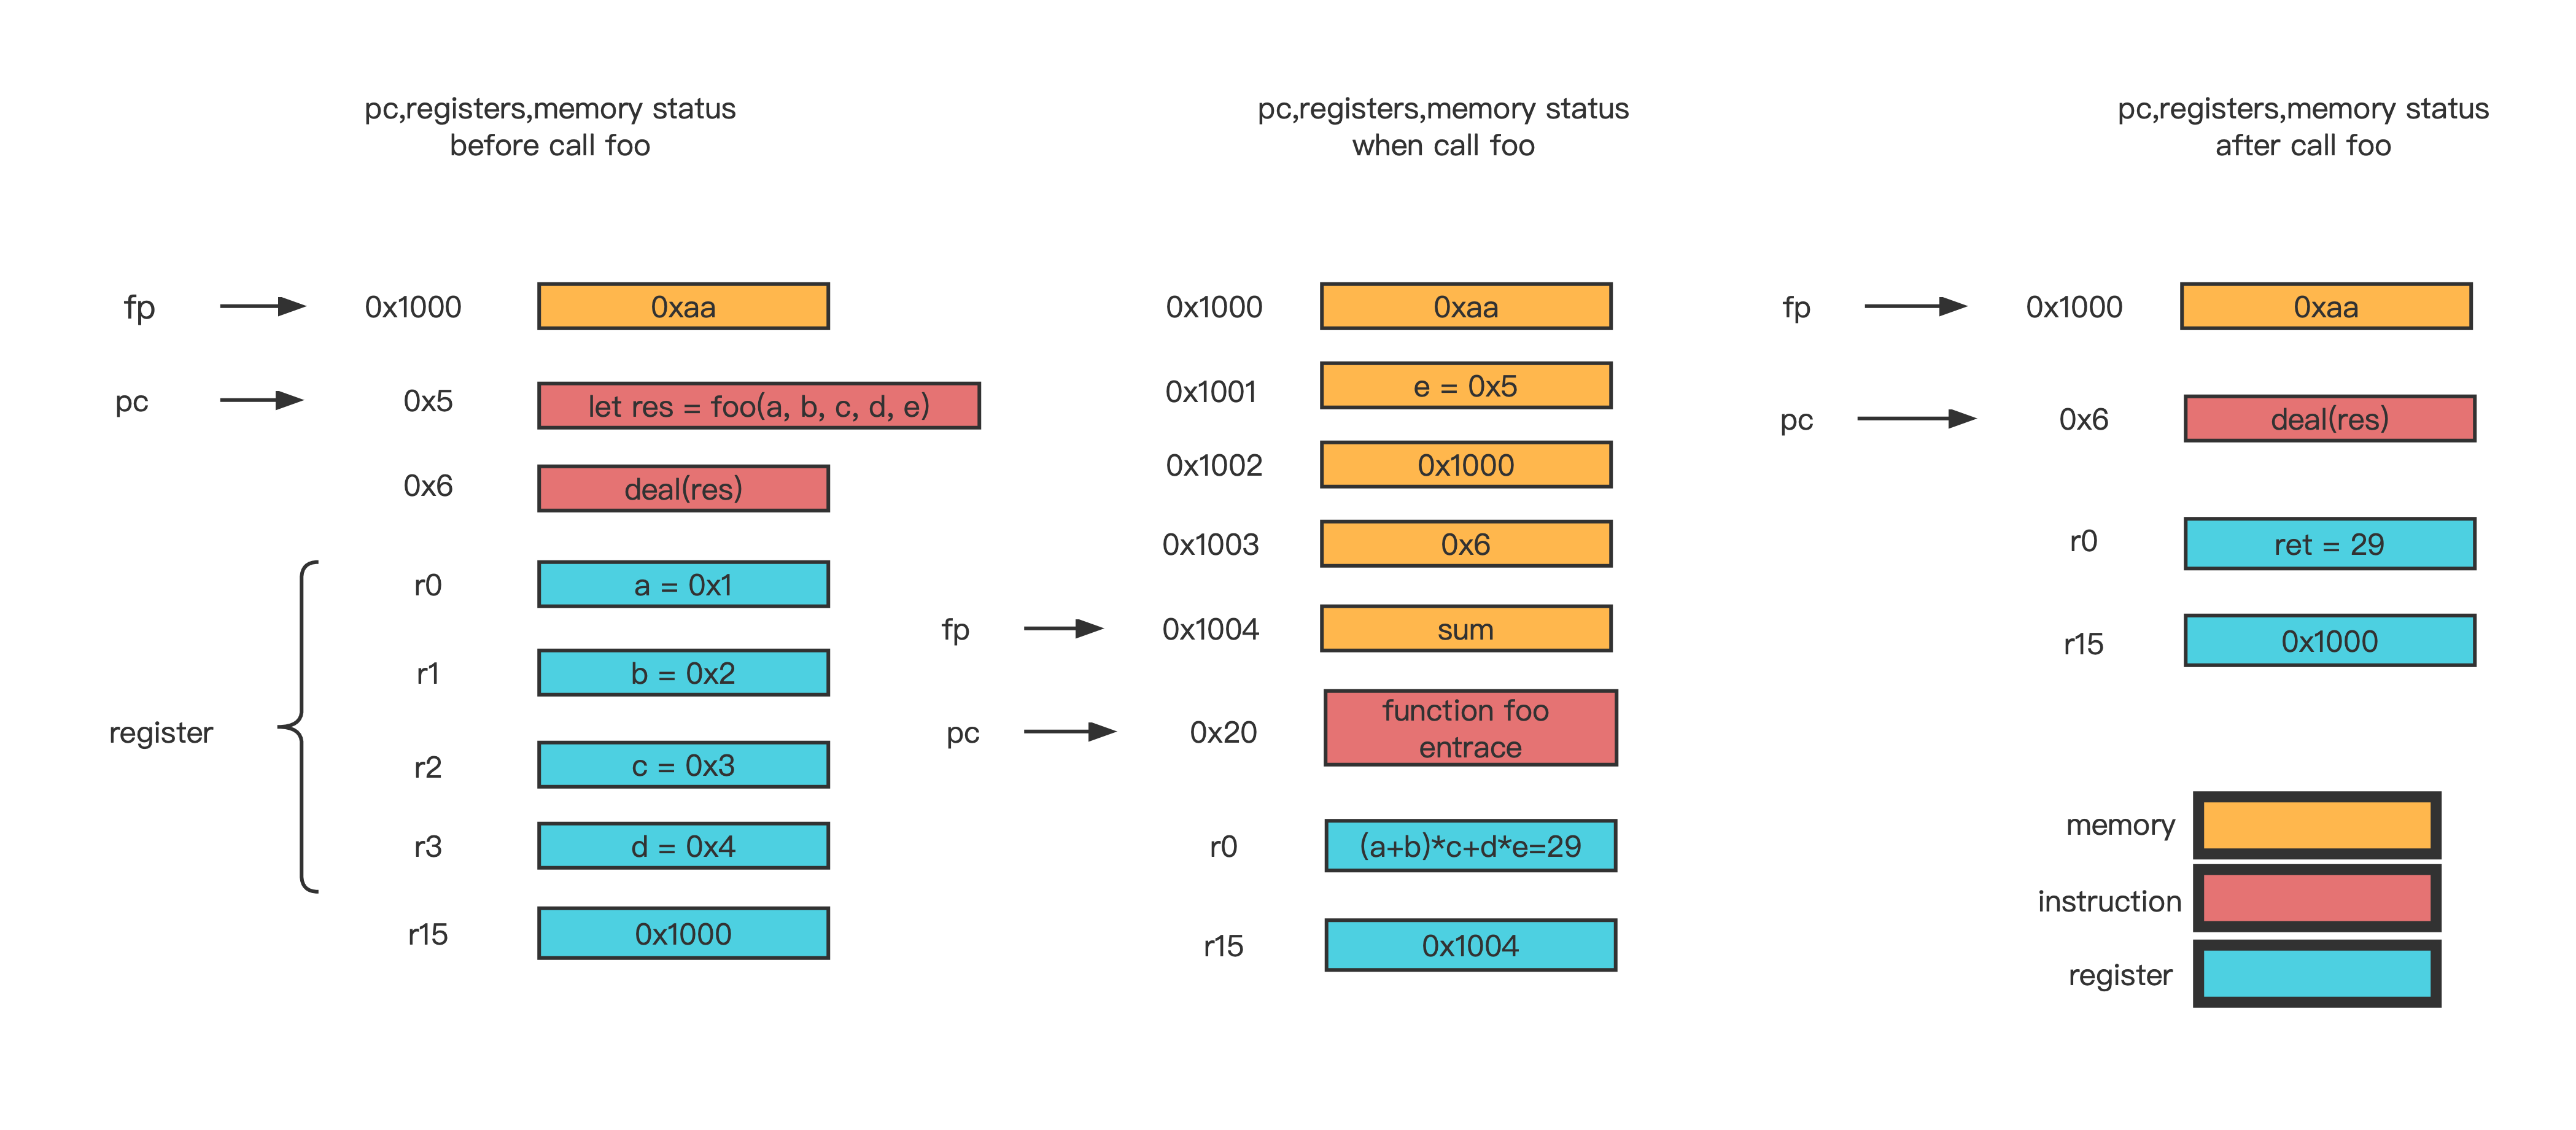
\includegraphics[width=1\textwidth]{olavm_procedure_call}
    \caption{OlaVM函数调用模型}
    \label{fig:processor call}
\end{figure}


